% {Descripción del artículo, no el resumen. Ventajas, desventajas, gráficas.}
El articulo \textit{Network analysis and link prediction in competitive women´s basketball} se centra en hacer predicción de resultados deportivos, en la primera división de la National Collegiate Athletic Association (NCAA) del baloncesto femenino de 2021 al 2024.

La idea central del articulo es que hace uso de estadísticas tradicionales, donde modela la dinámica deportiva del equipo, como pases, bloqueos y victorias; que no siempre se muestra toda la información disponible en estadísticas usuales, como las relaciones que existen entre las jugadoras y la influencia que tienen dentro de la cancha. 

El articulo trata de resolver el problema que al tener 2 equipos con estadísticas similares, estos se comporten de maneras totalmente distintas. Motivo por el cual hacen uso de una representación mediante grafos y una forma de medir esta interacción es mediante una puntuación, llamada Common Out-neighbor (CON) mostrando estos patrones competitivos entre equipos con estadísticas similares. 

Atravez del uso de una pagina llamada Page Rank, donde identifica la importancia de cada equipo. Posteriormente normalizan el CON y el Page Rank para construir un indice que llaman low-key leader strength.
$$\varepsilon_i=\text{CON}{i,\mathrm{norm}}-\text{PR}{i,\mathrm{norm}}.$$
Con esta metrica indican que equipos presentan patrones competitivos similares, en otras palabras buscan detectar equipos que se comportan como competidores fuertes sin ocupar todavía una posición destacada dentro de la red.
\begin{figure}[H]
    \centering
    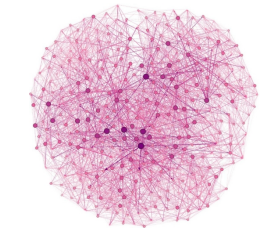
\includegraphics[width=0.5\linewidth]{imagenes/red_article_N_a.png}
    \caption{Imagen obtenida del articulo, donde se muestra la red formada de los partidos de la temporada 2023-2024}
    \label{fig:red_article}
\end{figure}
En el articulo tambien se analiza los pases que hay en la WNBA (Como la figura \ref{fig:pases_article}), dividen la cancha en 28 regiones donde se representan cada pase, como desventaja no se puede identificar que jugadora realizo el pase, solo identifican regiones dentro de la cancha, ademas de que esta red de pases fue construida atraves de 3 partidos, limitando el cmportamiento de la variedad de equipos que se encuentran presentes en la WNBA, lo que les limito la capacidad predictiva para la formacion de pases.
\begin{figure}[H]
    \centering
    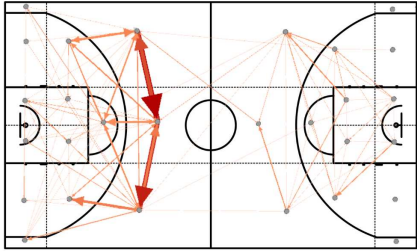
\includegraphics[width=0.5\linewidth]{imagenes/imagen_red_articulo_N_a.png}
    \caption{Imagen obtenida del articulo, en ella se muestran los pases de 3 partidos, mostrando las 28 regiones mas usuales}
    \label{fig:pases_article}
\end{figure}

Este articulo ayuda a identificar una metodologia util, para extraer informacion, que no esta presente en estadisticas tradicionales, sinembargo el conjunto de datos limitados usado representa una limitante en la aplicacion de la seleccion de alineaciones.


\cite{bonato2026networkanalysislinkprediction}